\documentclass{beamer}
 
\usetheme{metropolis}
\usepackage[utf8]{inputenc}

%Information to be included in the title page:
\title{Benchmarking framework for real-time operating system applications}
\subtitle{Study and implementation with Contiki and Riot}
\author{Julien Gomez \and Trong-Vu Tran}
\institute{Université catholique de Louvain}
\date{\today}

\begin{document}

%%%%

\frame{\titlepage}

%%%
\begin{frame}{}
\protect\hypertarget{embedded-systems}{}
\begin{center}
  \LARGE 1,000,000,000,000
\end{center}

\end{frame}
%%%

\begin{frame}{Objectives}
\protect\hypertarget{objectives}{}

\begin{itemize}
\tightlist
\item
  Theoretical summary
\item
  Benchmarking tool
\end{itemize}

\end{frame}

%%%

\begin{frame}{Theory}
\protect\hypertarget{theory}{}

TODO Mindmap here

\end{frame}

%%%

\hypertarget{public-support-and-interest}{%
\section{Public support and interest}\label{public-support-and-interest}}

\begin{frame}{Benchmarking tool for RTOS applications}
\protect\hypertarget{benchmarking-tool-for-rtos-applications}{}

TODO source

\end{frame}

%%%

\begin{frame}{Interest of the community}
\protect\hypertarget{interest-of-the-community}{}

RIOT Summit 2018

\end{frame}

%%%

\begin{frame}
  \begin{figure}
    \centering
    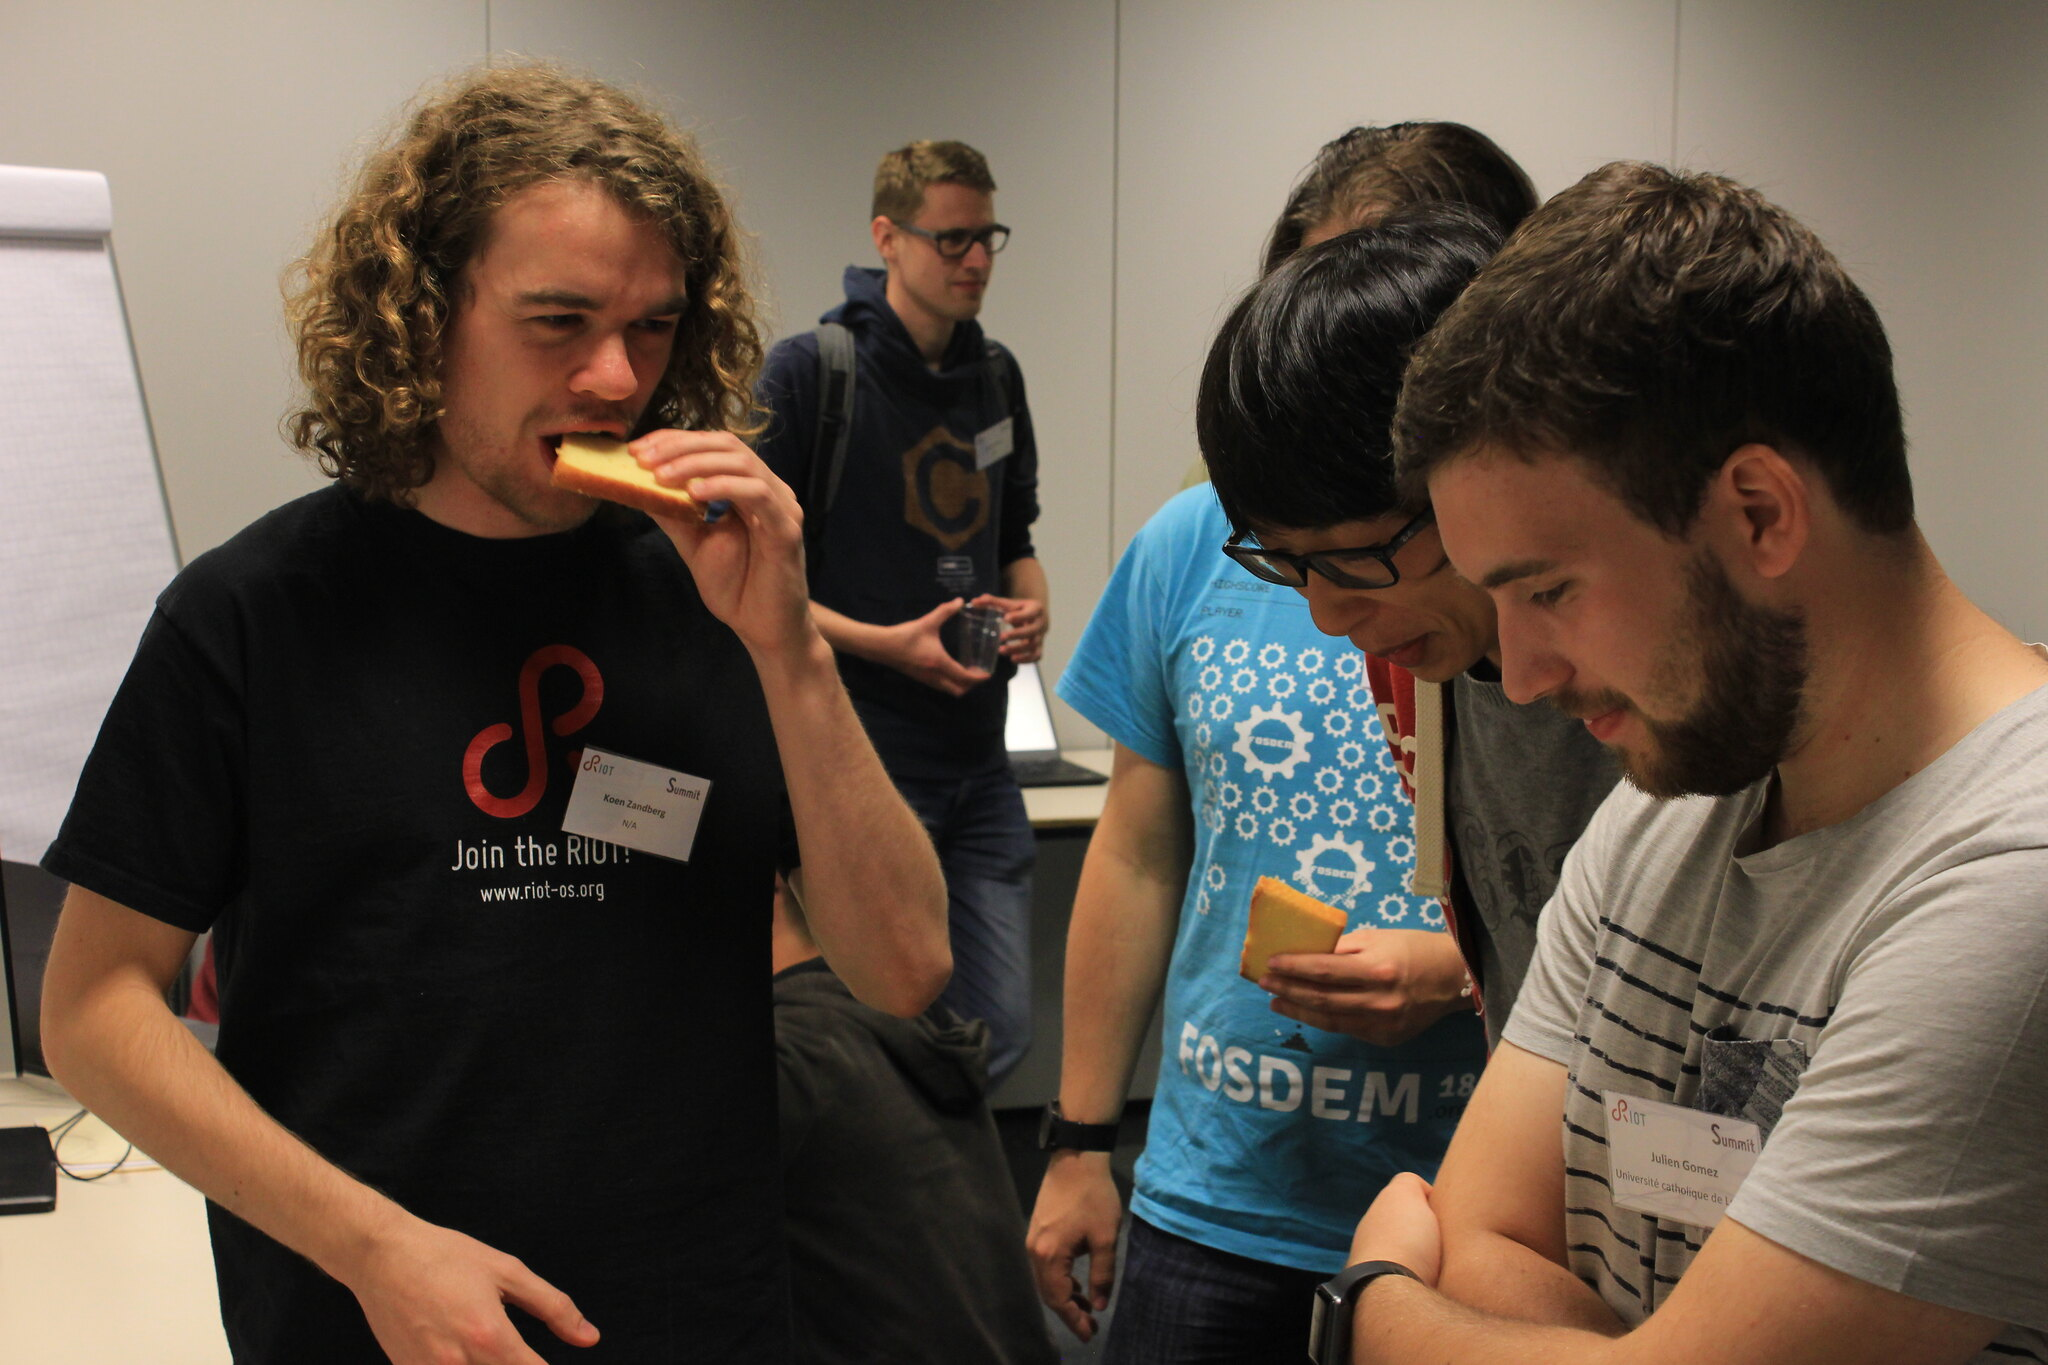
\includegraphics[scale=0.15]{assets/riotsummit.jpg}
    %\caption{}
    \end{figure}
\end{frame}

%%%

\begin{frame}{Contact with the communities}
\protect\hypertarget{contact-with-the-communities}{}

\begin{itemize}
\tightlist
\item RIOT
\item Contiki
\item FreeRTOS
\item Apache MyNewt
\item mBed
\item /r/embedded
\end{itemize}
\tightlist
\end{frame}

%%%

\hypertarget{developpement-and-implementation}{%
\section{Developpement and implementation}\label{developpement-and-implementation}}

\begin{frame}{Benchmark definition}
\protect\hypertarget{benchmark-definition}{}

\begin{quote}
``A tool designed to assess the performances of a system.''
\end{quote}

In our case, a benchmarking tool to assess the performances of
applications running on different RTOS.

\end{frame}

%%%

\begin{frame}{RTOS}
\protect\hypertarget{rtos}{}

\begin{block}{Contiki}

\begin{itemize}
\tightlist
\item
  Cooperative scheduling
\item
  Event-driven
\end{itemize}

\end{block}

\begin{block}{RIOT}

\begin{itemize}
\tightlist
\item
  Preemptive scheduling
\item
  Multithreading
\end{itemize}

\end{block}

\end{frame}

%%%

\begin{frame}{Metrics}
\protect\hypertarget{metrics}{}

\begin{block}{Framework metric}

\begin{itemize}
\tightlist
\item
  Context switching time
\end{itemize}

\end{block}

\begin{block}{Other metrics}

\begin{itemize}
\tightlist
\item
  Interrupt latency
\item
  Memory usage
\item
  Power consumption
\end{itemize}

\end{block}

\end{frame}

%%%

% \begin{frame}{Multiple approaches}
% \protect\hypertarget{multiple-approaches}{}

\begin{frame}{Kernel approach}

Implementing the framework in the RTOS kernel.

\begin{itemize}
\tightlist
\item
  Tedious approach
\item
  Strongly platform-dependent
\end{itemize}

\end{frame}

%%%

\begin{frame}{Extension approach}

Implementing the framework as a RTOS extension.

\begin{itemize}
\tightlist
\item
  Contiki app and RIOT module
\item
  Internal clock
\end{itemize}

\end{frame}

%%%

\begin{frame}{Devices approach}

Implementing the framework with external devices.

\begin{itemize}
\tightlist
\item
  Pocket Science Lab board to measure the context switching time
\item
  Laptop to communicate with the PSLab
\end{itemize}

\end{frame}

%%%

\hypertarget{results}{%
\section{Results}\label{results}}

%%%

\begin{frame}{Performances gathering}
\protect\hypertarget{performances-gathering}{}

\begin{itemize}
\tightlist
\item
  Reference value
\item
  Oscilloscope
\end{itemize}

\end{frame}

%%%

\begin{frame}

\begin{figure}
\centering
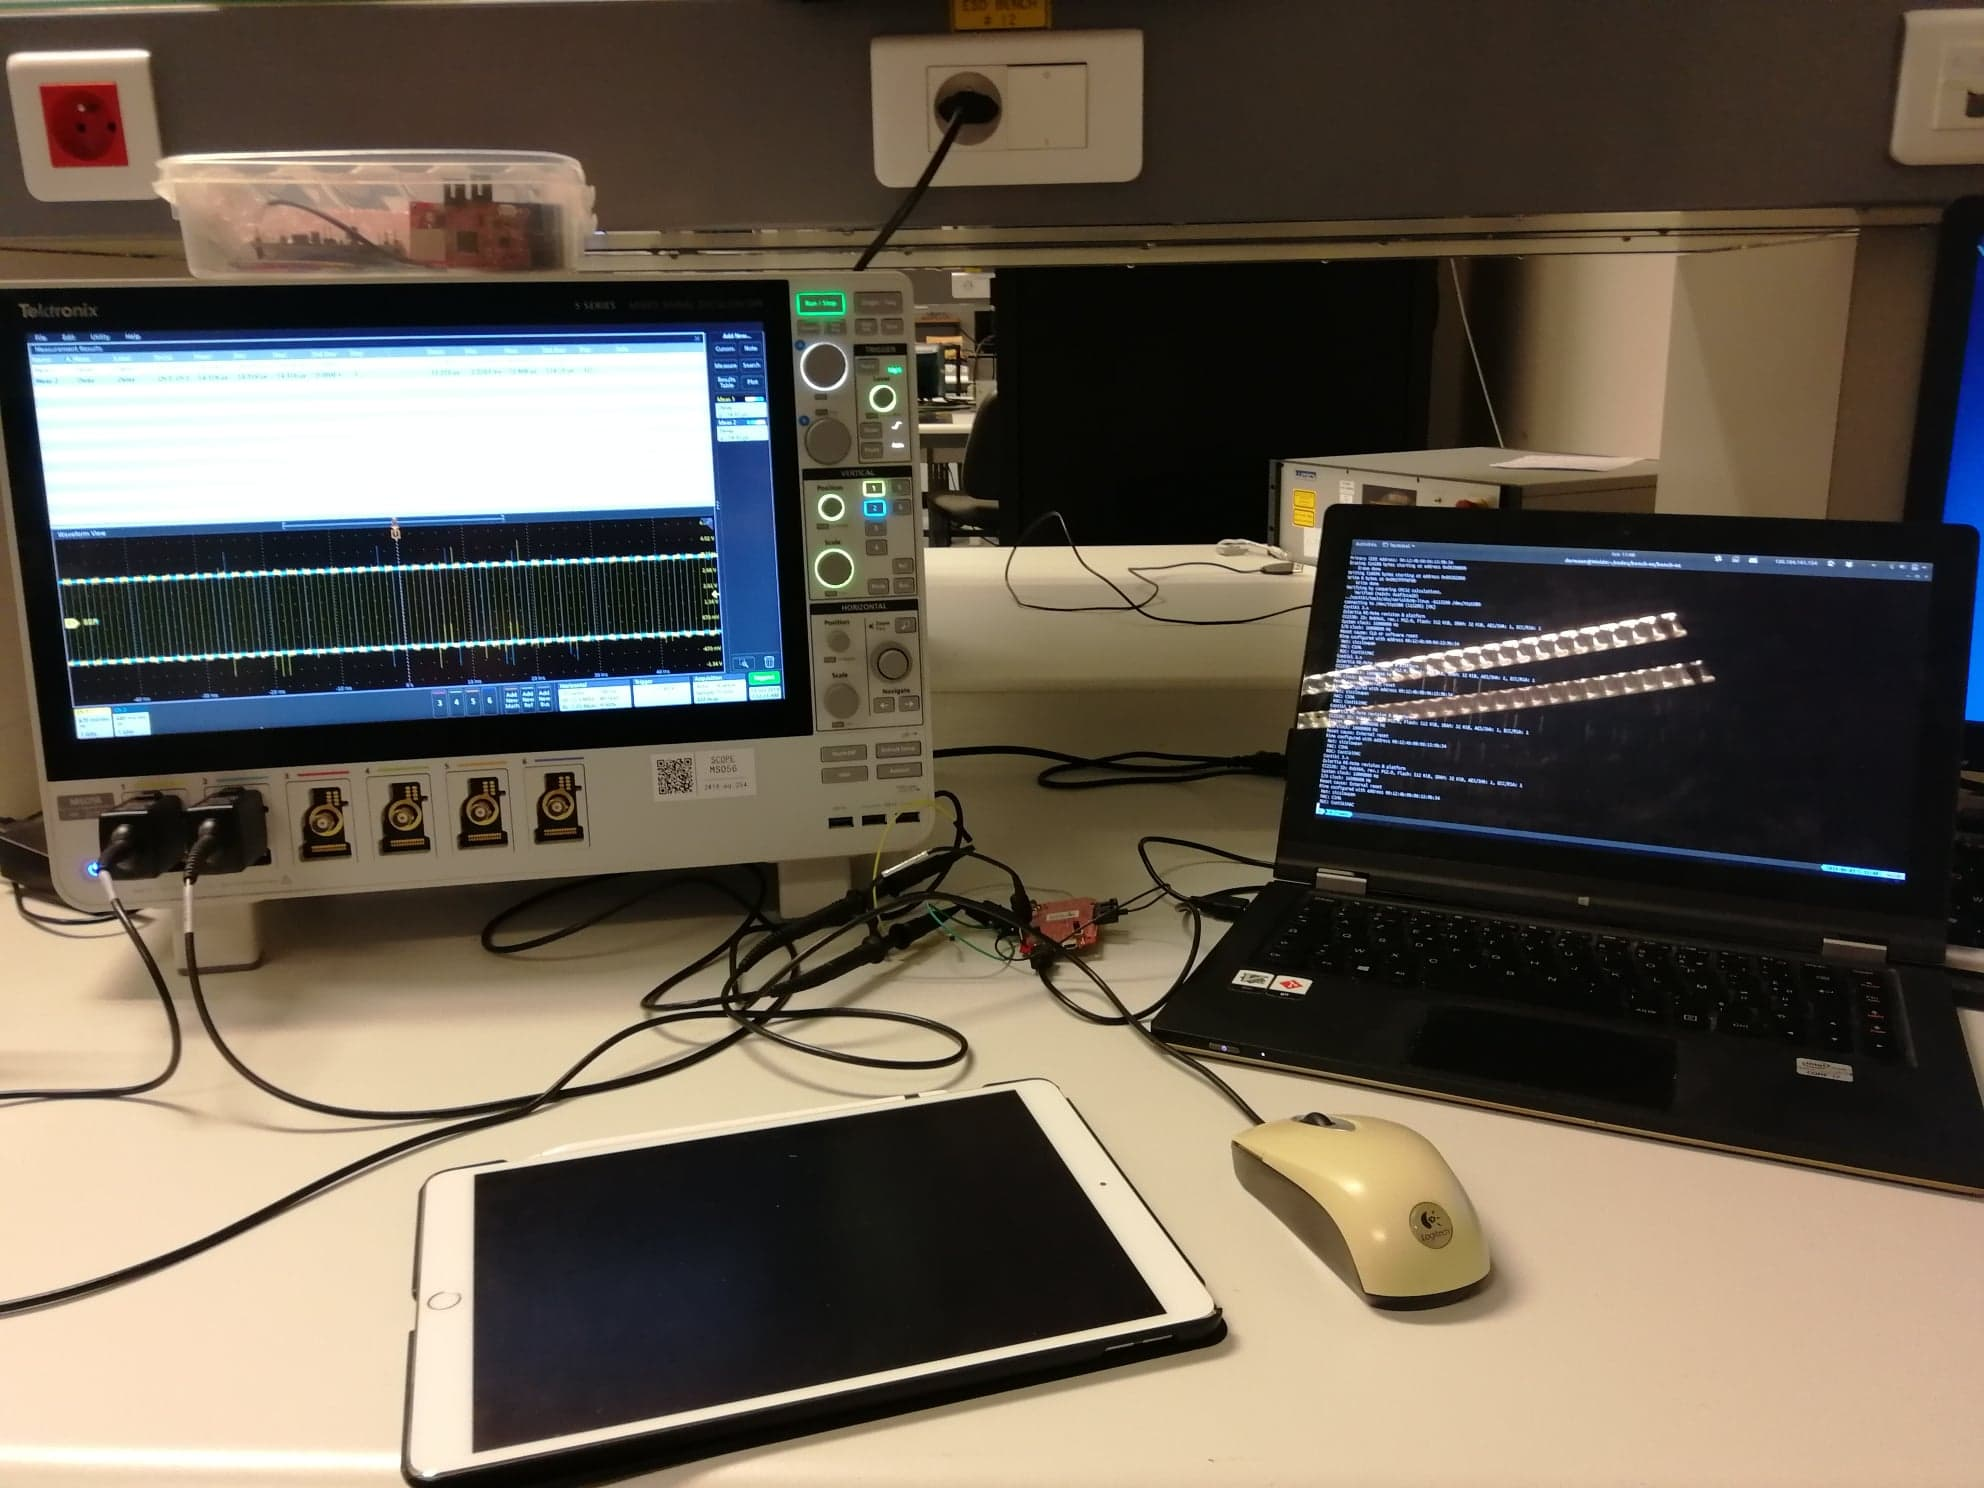
\includegraphics[scale=0.1]{assets/1.jpg}
\caption{oscilloscope setup}
\end{figure}

\end{frame}

%%%

\begin{frame}{Overhead measurements}
  \protect\hypertarget{overhead-measurements}{}
  \begin{figure}
    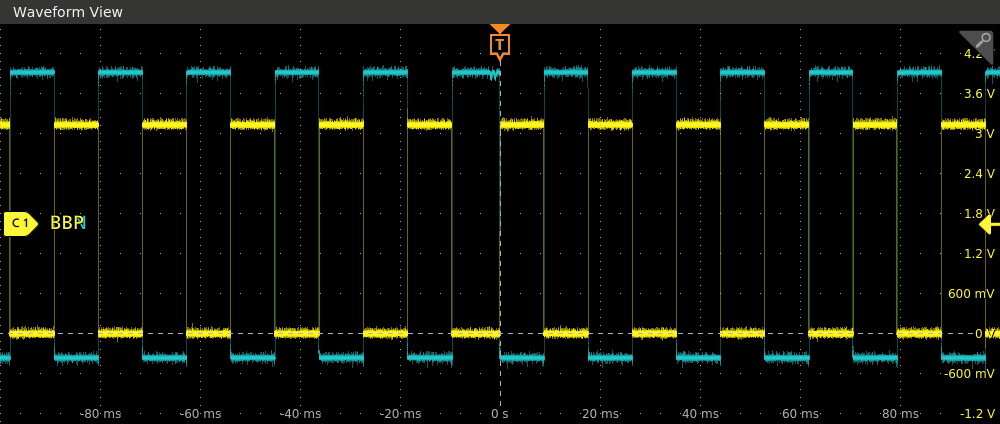
\includegraphics[scale=0.4]{assets/reference-value-overhead-contiki-z1.png}
    \caption{reference value overhead (Contiki on Z1 board)}
  \end{figure}
\end{frame}
  
  %%%
  
\begin{frame}
  \begin{figure}
    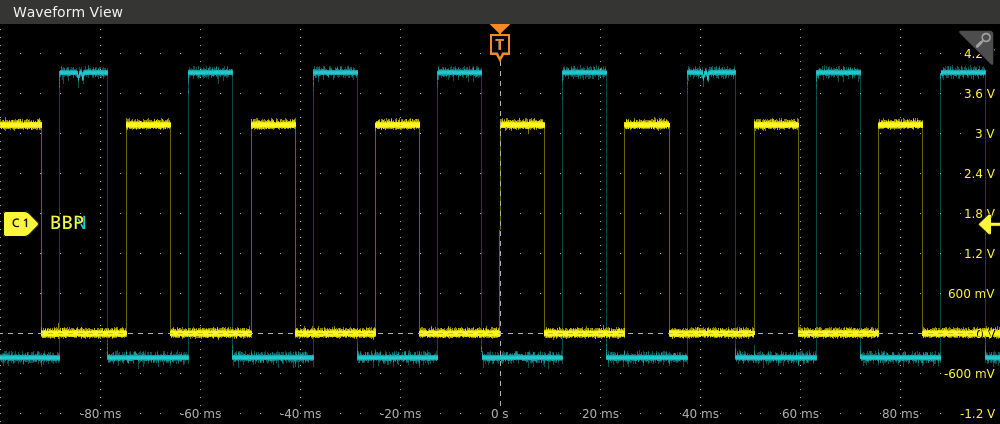
\includegraphics[scale=0.4]{assets/extension-framework-overhead-contiki-z1.png}
    \caption{extension framework overhead (Contiki on Z1 board)}
  \end{figure}
\end{frame}
  
  %%%
  
\begin{frame}
  \begin{figure}
    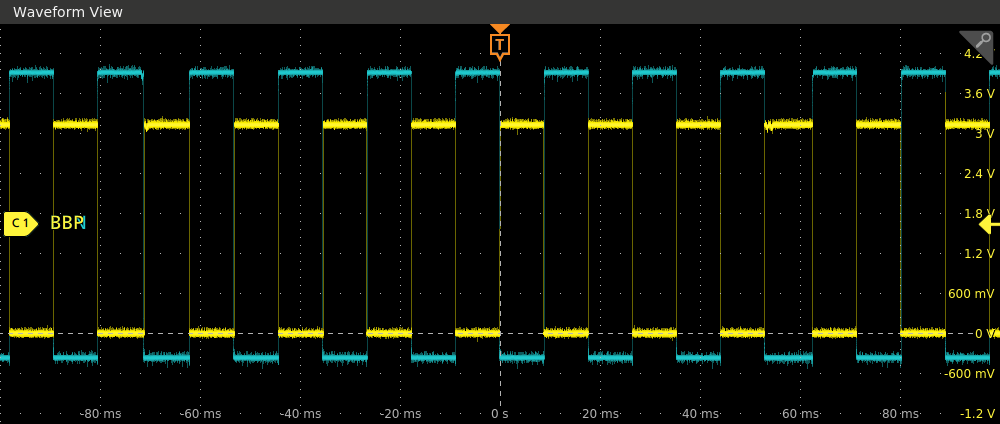
\includegraphics[scale=0.4]{assets/devices-framework-overhead-contiki-z1.png}
    \caption{Devices framework overhead (Contiki on Z1 board)}
  \end{figure}
\end{frame}
  
  %%%

\begin{frame}{Framework measurements}
  \protect\hypertarget{framework-measurements}{}
  \begin{figure}
    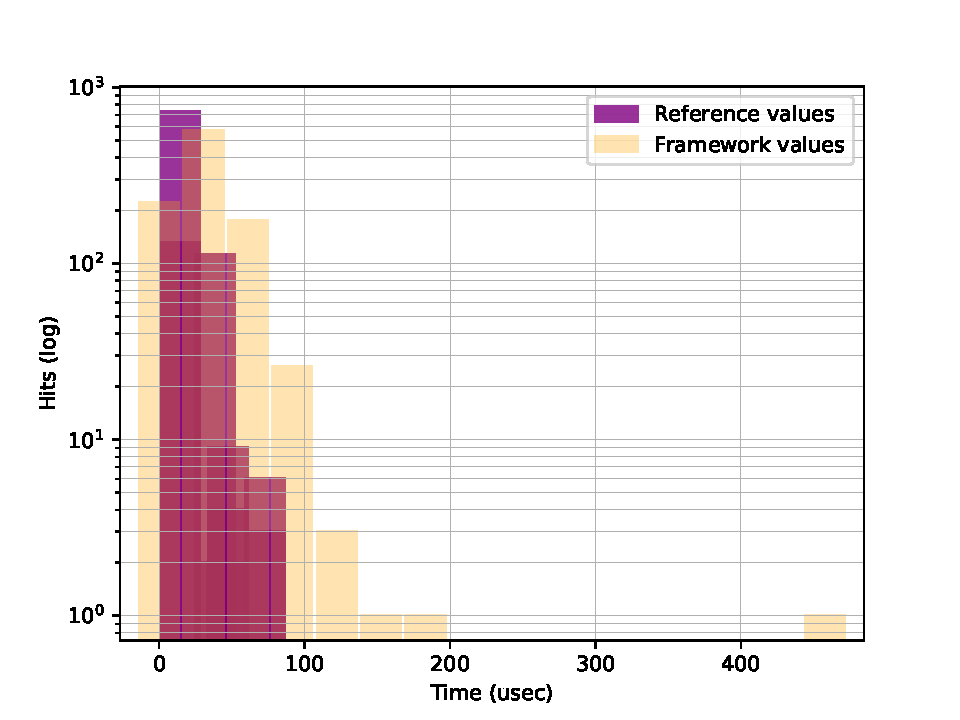
\includegraphics[scale=0.4]{assets/comparison-extension-framework-contiki-remote.pdf}
    \caption{Extension framework (Contiki on RE-Mote)}
  \end{figure}
\end{frame}

\begin{frame}
  \begin{figure}
    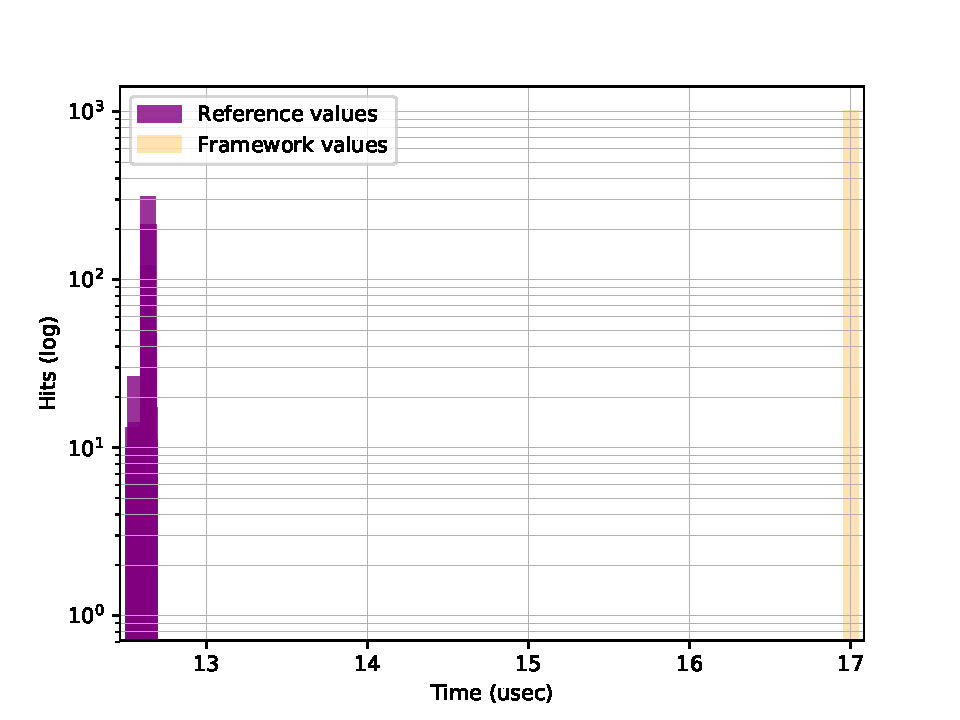
\includegraphics[scale=0.4]{assets/comparison-extension-framework-riot-remote.pdf}
    \caption{Extension framework (RIOT on RE-Mote)}
  \end{figure}
\end{frame}

\begin{frame}
  \begin{figure}
    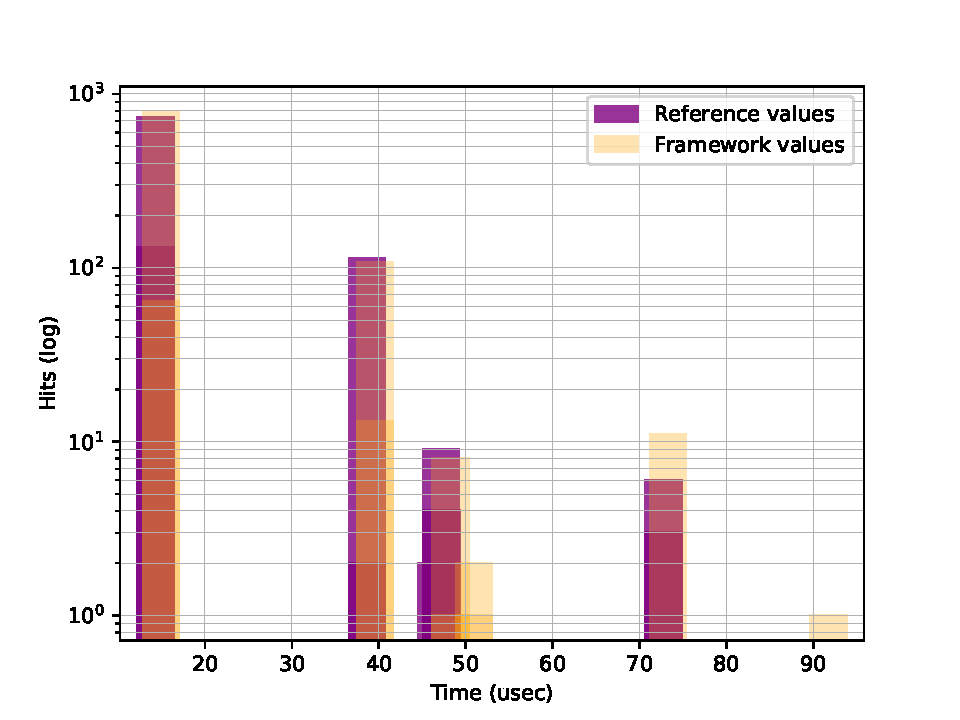
\includegraphics[scale=0.4]{assets/comparison-devices-framework-contiki-remote.pdf}
    \caption{Devices framework (Contiki on RE-Mote)}
  \end{figure}
\end{frame}

\begin{frame}
  \begin{figure}
    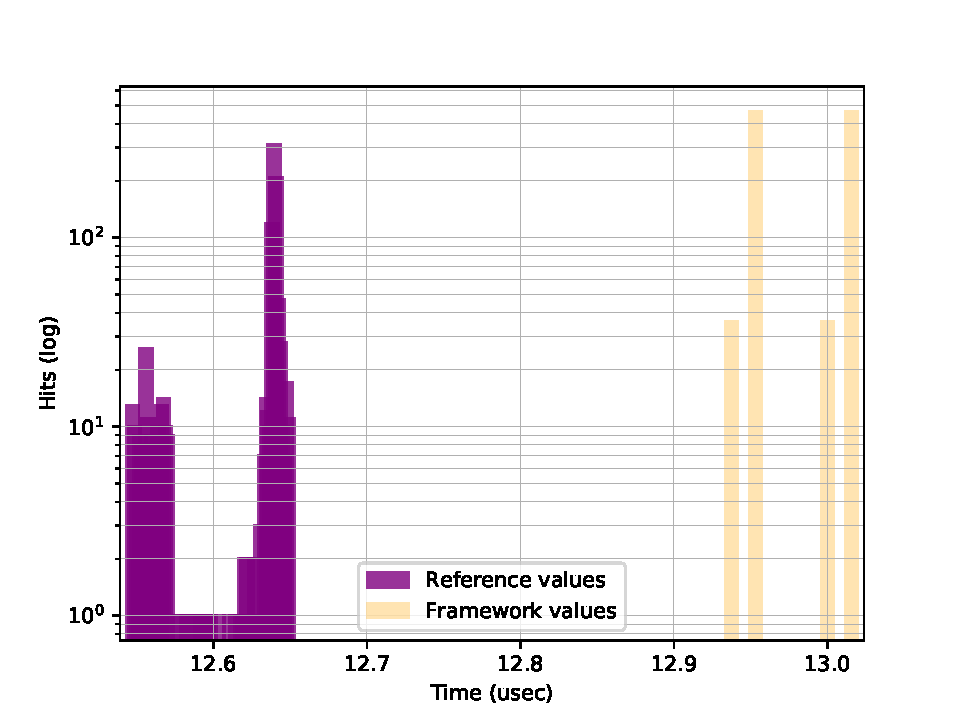
\includegraphics[scale=0.4]{assets/comparison-devices-framework-riot-remote.pdf}
    \caption{Devices framework (RIOT on RE-Mote)}
  \end{figure}
\end{frame}

%%%

\hypertarget{conclusion}{%
\section{Conclusion}\label{conclusion}}

%%%

\begin{frame}{Future possible improvements}
  \protect\hypertarget{future-possible-improvements}{}
  
  \begin{itemize}
  \tightlist
  \item
    Add metrics
  \item
    Improve the devices framework
  \end{itemize}
\end{frame}

%%%

\begin{frame}{Parallel works}
\protect\hypertarget{parallel-works}{}

Embench (June 11th, 2019)

\end{frame}

%%%

\begin{frame}

Embench: Recruiting for the Long Overdue and Deserved Demise of
Dhrystone as a Benchmark for Embedded Computing by Prof David Patterson

\end{frame}

%%%

\begin{frame}{Demonstration}
\protect\hypertarget{demonstration}{}

TODO video ou live demo

\end{frame}

%%%

\begin{frame}

\begin{figure}
\centering
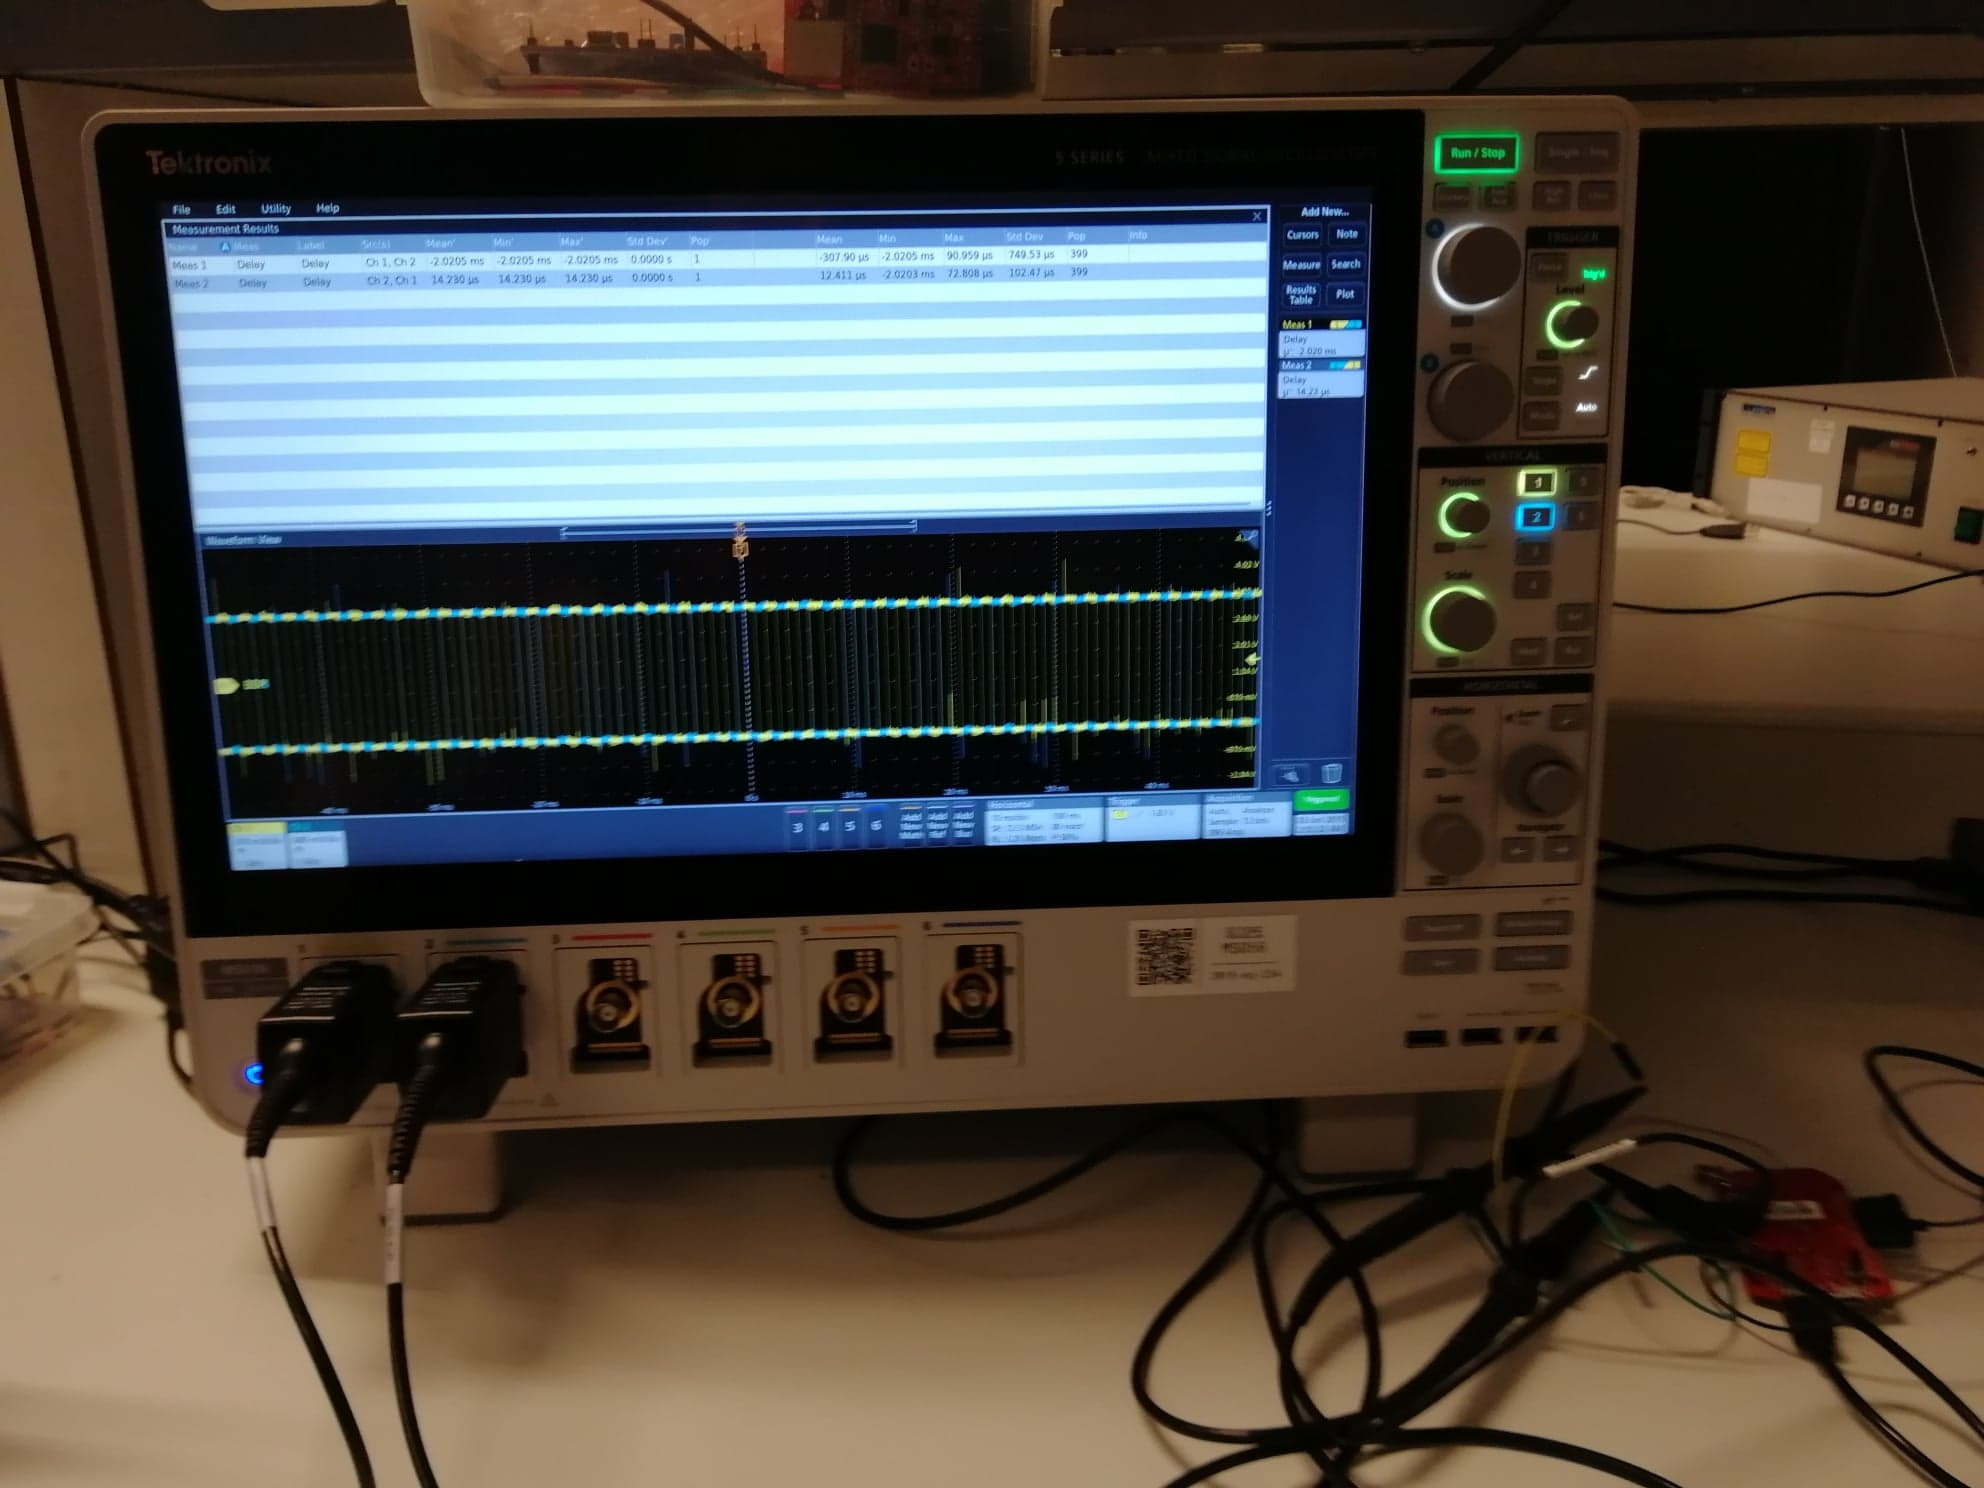
\includegraphics[scale=0.1]{assets/2.jpg}
\caption{more oscilloscope setup}
\end{figure}

\end{frame}

%%%

\begin{frame}

\begin{figure}
\centering
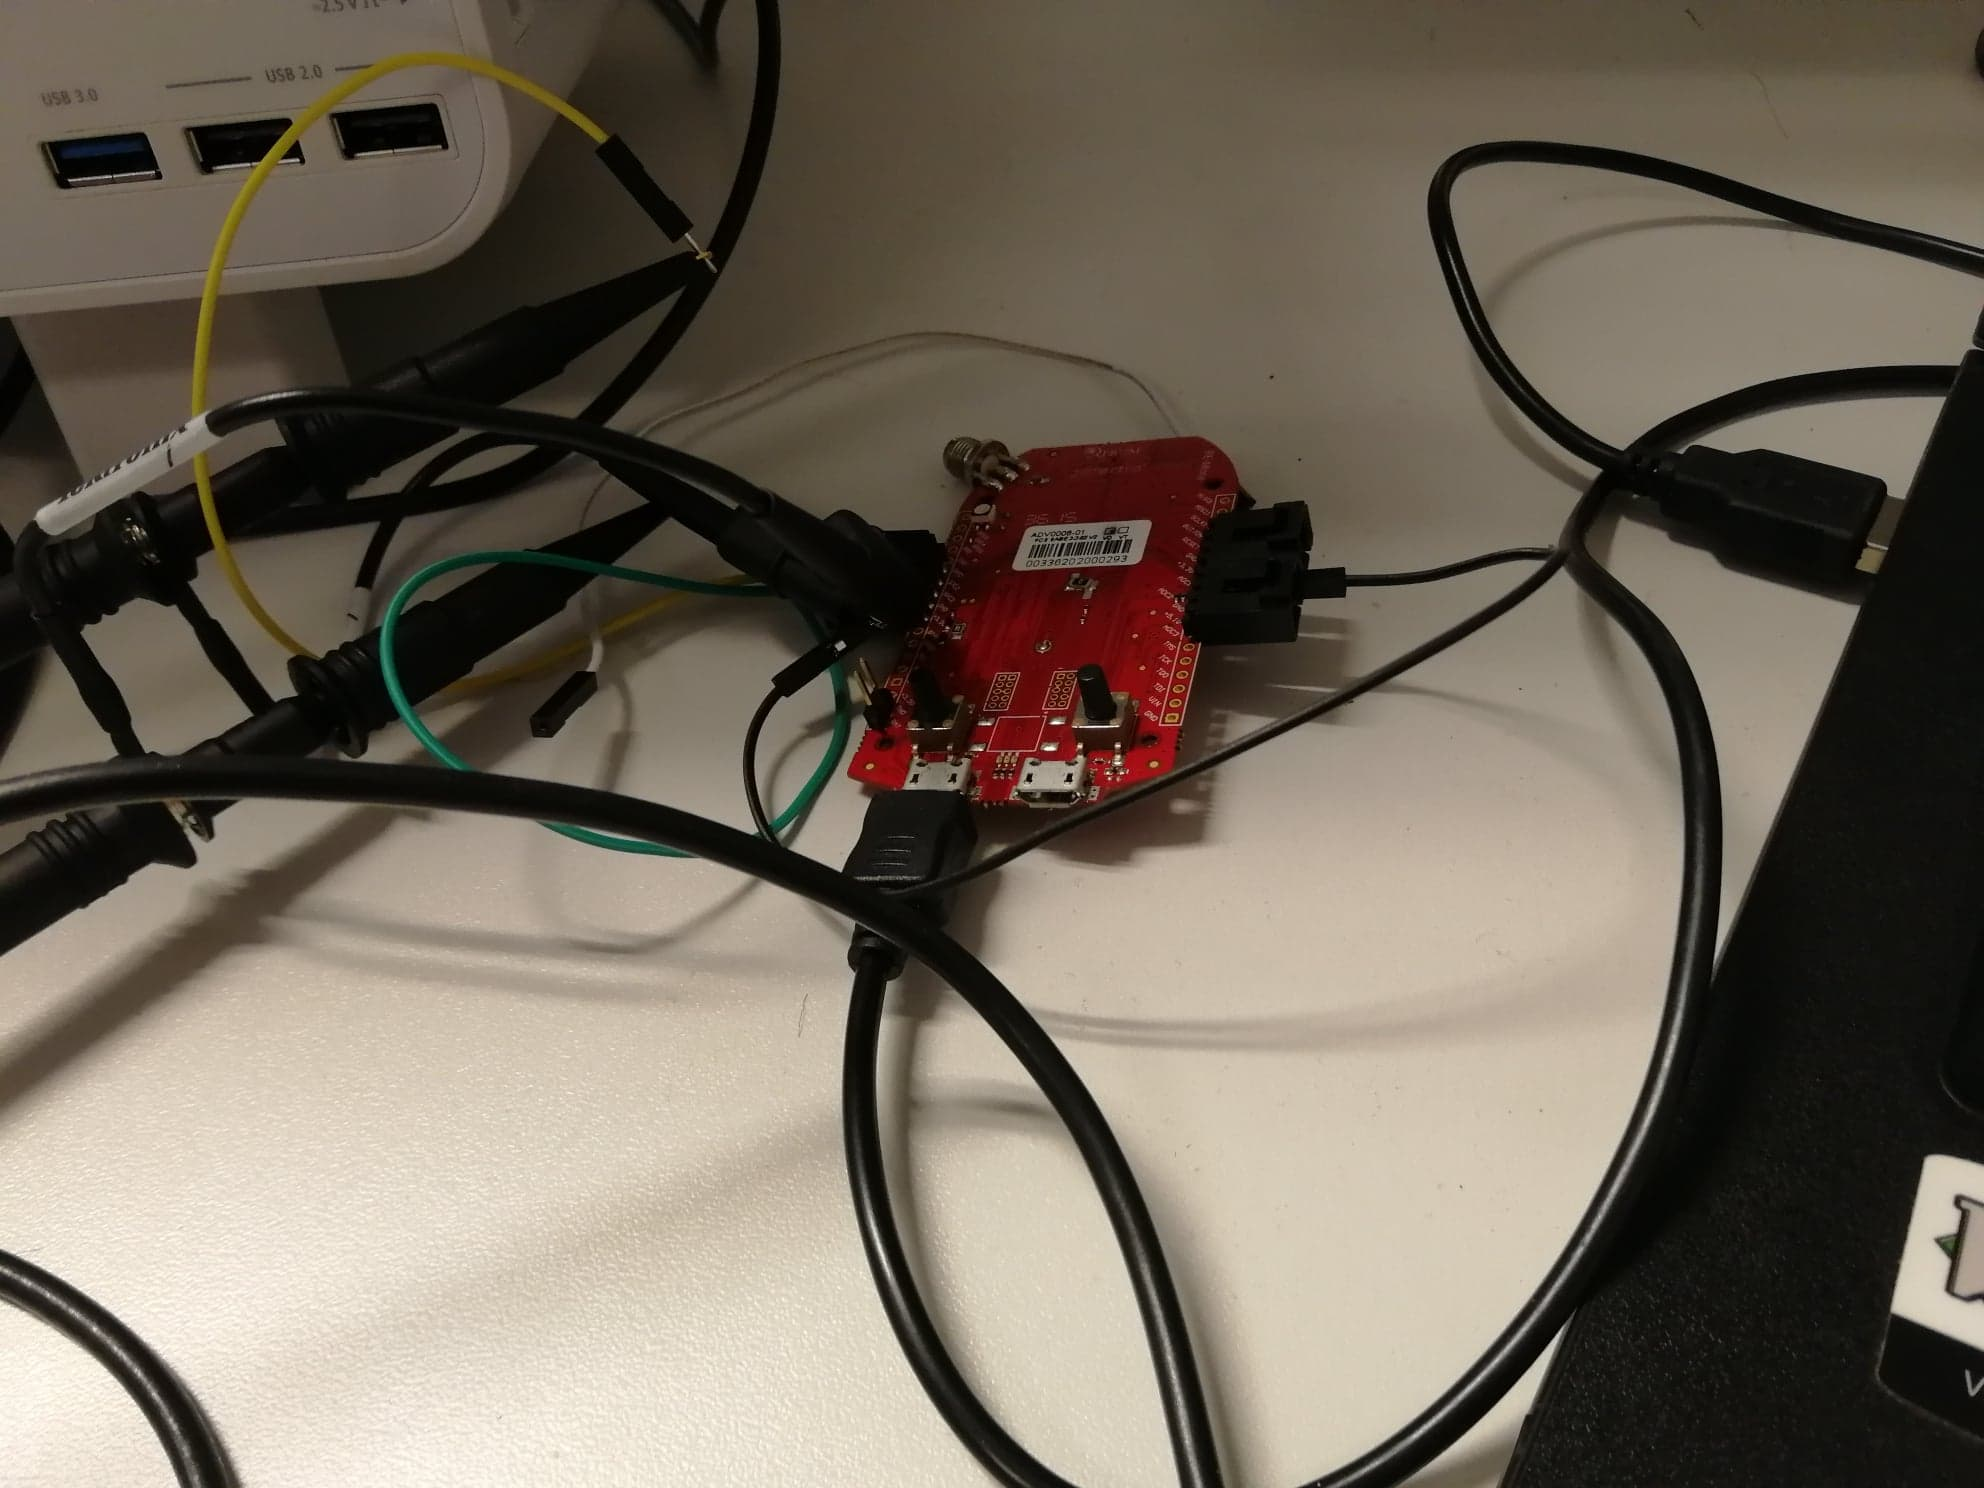
\includegraphics[scale=0.1]{assets/3.jpg}
\caption{more oscilloscope setup}
\end{figure}

\end{frame}

%%%

\end{document}